\subsection{The MCU and its Auxiliary Circuits}
\label{subsec:mcu_design}
Designing the \acs{mcu} and its auxiliary circuits is based on the STM32F405 datasheet\cite{stmicro_stm32f405xx_2020} and on an example design by Philip Salmony described in a YouTube video\cite{salmony_kicad_2020}.
Apart from different stepper motor driver \acs{ic} connections, there are only minor differences between the hardware revisions.

The design follows closely the video, as its development approach seems sound.
First, the preliminary design is done using the STM32CubeMX tool.
The tool allows users to select the target \acs{mcu} and graphically assign alternate functions to pins (each \acs{gpio} pin on an STM32 features multiple alternate functions, connecting for example \acs{spi} bus to the pin).
Given that some internal \acs{mcu} peripherals can be connected to multiple \acs{gpio}s and alternate functions, it is also possible to optimize the design and wiring based on the preliminary layout of the \acs{pcb} by changing alternate function assignments.
The assigned alternate functions to the \acs{mcu} for the revision 2 of the hardware can be seen in the Figure~\ref{fig:cubemx}.
The STM32CubeMX is also capable of setting up the peripherals and can generate initialization code for the peripherals and whole C/C++ project with everything set-up.

\begin{figure}[H]
    \centering
    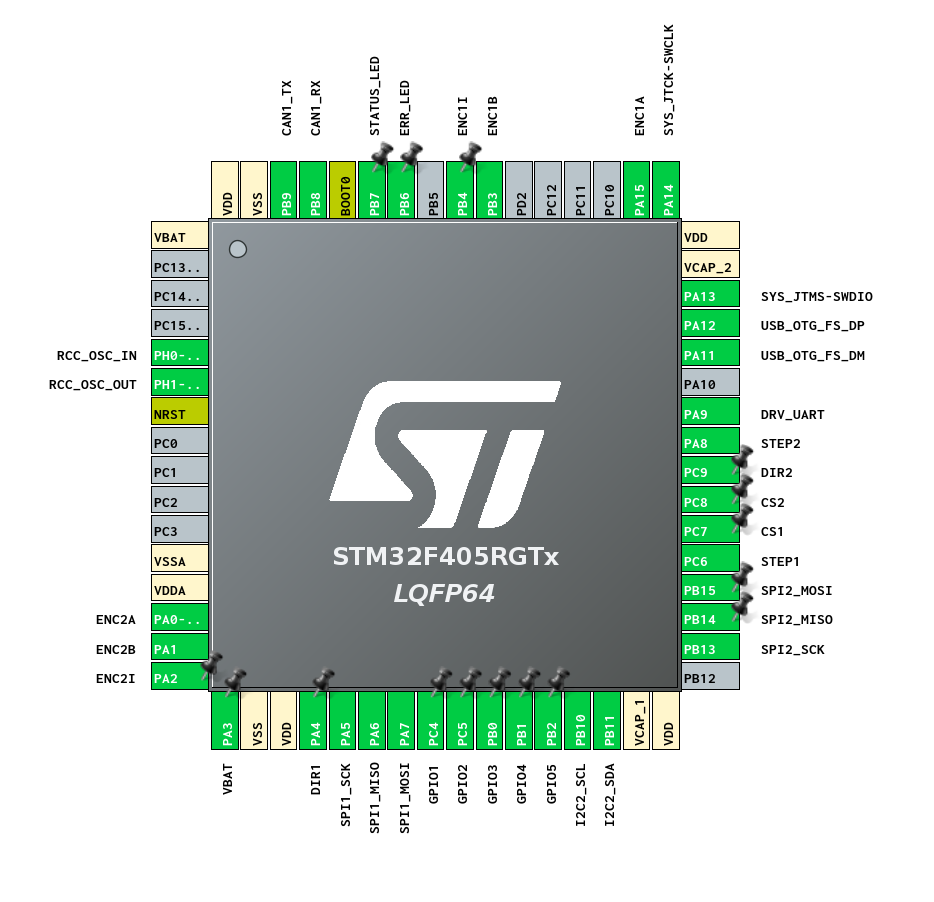
\includegraphics[width=0.9\textwidth]{obrazky/cube_mx}
    \caption{Designing the MCU connections using STM32CubeMX.}
    \label{fig:cubemx}
\end{figure}

After the pin and alternate functions assignment was done, we used the information from the datasheet to design the \acs{mcu} circuitry itself.
The electronic schematic can be seen in the Figure~\ref{fig:schem_mcu}, there are not that many components in this part of the schematic, there are only two \textbf{VCAP} capacitors with values taken from the datasheet~\cite{stmicro_stm32f405xx_2020}.
Furthermore, there are net labels connected to other parts of the schematic.

\begin{figure}[H]
    \centering
    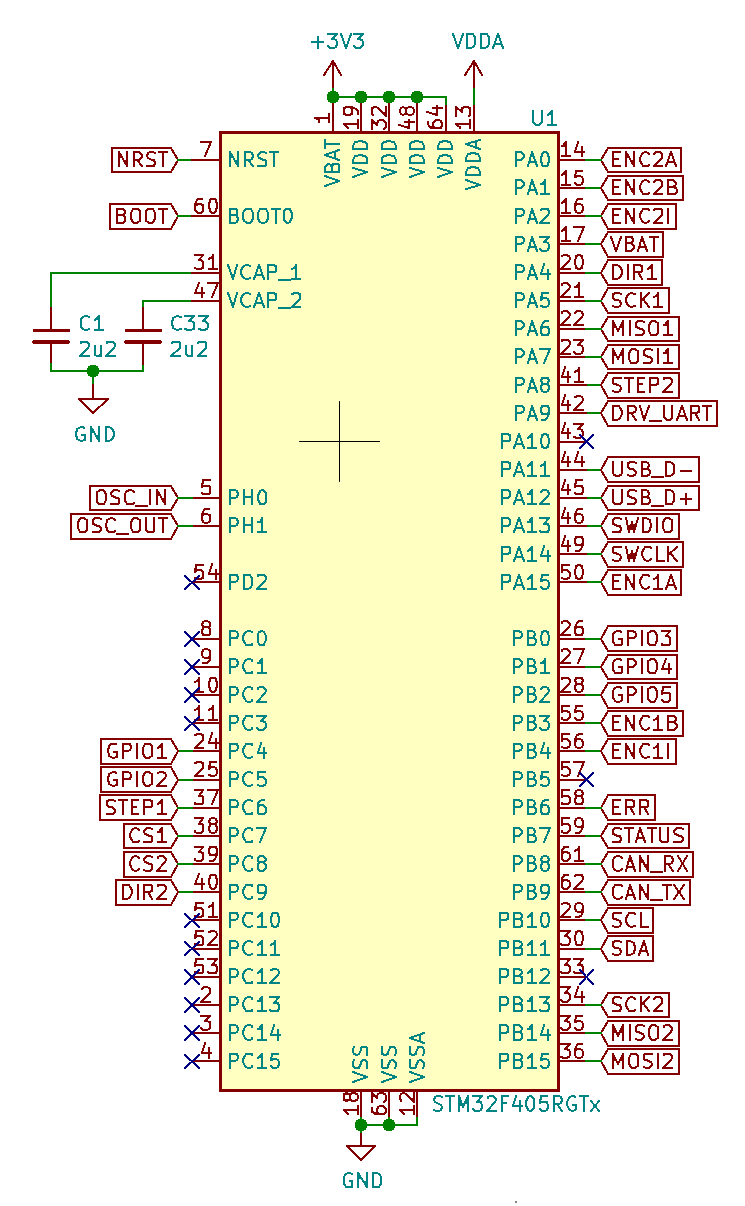
\includegraphics[width=0.6\textwidth]{obrazky/schem_mcu}
    \caption{The MCU schematic.}
    \label{fig:schem_mcu}
\end{figure}

More interesting parts of the \acs{mcu} schematic are the auxiliary circuits shown in the Figures~\ref{fig:schem_mcu_power} and~\ref{fig:schem_mcu_aux}.
The Figure~\ref{fig:schem_mcu_power} depicts the power supply filtering circuits.
As per the datasheet\cite{stmicro_stm32f405xx_2020}, for each \textbf{VDD} there should be a 100~nF capacitor and there should be a single 4.7~uF capacitor on the rail.

As for the analog filtering circuit, a simple low-pass filter utilizing a ferrite bead was employed as can be seen in the Figure~\ref{fig:schem_mcu_power}, the circuit was taken from the example project\cite{salmony_kicad_2020}.

\begin{figure}[H]
    \centering
    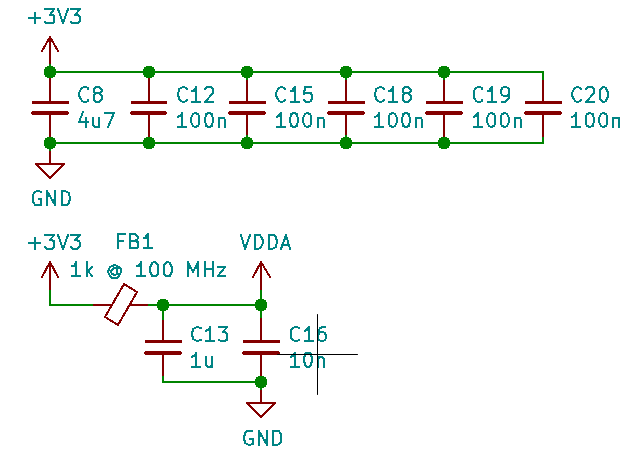
\includegraphics[width=0.5\textwidth]{obrazky/schem_mcu_power_filter}
    \caption{The MCU power supply filtering schematic.}
    \label{fig:schem_mcu_power}
\end{figure}

The Figure~\ref{fig:schem_mcu_aux} shows other \acs{mcu} auxiliary circuits - boot mode selection, reset and external crystal oscillator.
The boot mode selection consists of an \acs{spdt} (\acl{spdt}) switch that connects the \textbf{BOOT0} \acs{gpio} to either 3.3~V or \acs{gnd} through a 10 k\textohm resistor.
Pulling the \textbf{BOOT0} down to \acs{gnd} enables normal boot, where the \acs{mcu} starts the controller's firmware, on the other hand pulling the pin up to the 3.3~V makes the \acs{mcu} boot its bootloader, and it can be programmed using the \acs{dfu} protocol via \acs{usb}.

The reset pin on the schematic is connected to a jumper with a small filtering capacitor of 10~nF for debouncing.
A pull-up resistor required for the reset to work is already included in the \acs{mcu} therefore an external one is not required.

The external crystal clock is required for \acs{usb} to work.
In our case, we utilized the oscillator circuit used in the example project, where we kept the value of the load capacitor of 12~pF, ignoring the stray capacity of the \acs{pcb}, for improved performance of the oscillator, the following equation may be utilized to compute the load capacitance.

\begin{equation}
    \centering
    C_{load} = 2 * (C_{load-{datasheet}} - C_{stray})
    \caption{Oscillator load capacitance calculation\cite{salmony_kicad_2020}.}
    \label{eq:clock_cap}
\end{equation}

In the equation, the $C_{load-{datasheet}}$ is the load capacitance specified by the datasheet, and the $C_{stray}$ is the stray capacitance of the \acs{pcb}.
The feed resistor value was also used as it was in the example project, but the specific value calculation can be found in the Application Note AN2867\cite{stmicro_an2867_2020}.

\begin{figure}[H]
    \centering
    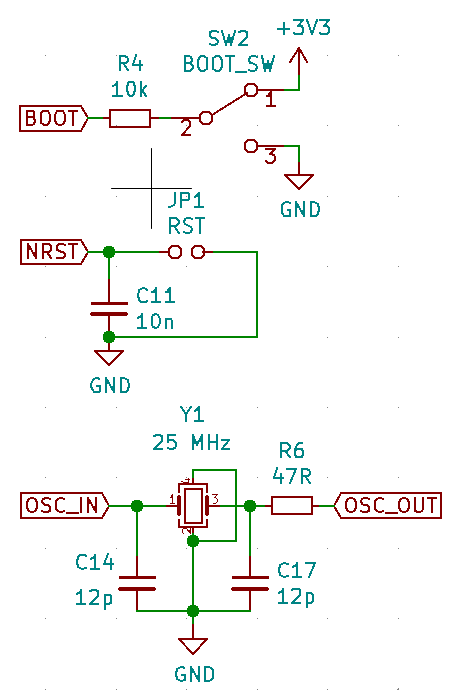
\includegraphics[width=0.4\textwidth]{obrazky/schem_mcu_aux}
    \caption{Auxiliary circuits for the MCU - boot mode, reset and oscillator.}
    \label{fig:schem_mcu_aux}
\end{figure}

\subsection{Power System}
\label{subsec:power_system}
As was discussed in the Section~\ref{subsubsec:power_design}, the power system consists of two rails - the power electronics rail and the 5~V rail for the \acs{mcu} and supplementary circuits.
In both cases, the rail should be filtered and should employ some safety features.

As for the power electronics rail, only input voltage filtering using capacitors was utilized.
The main reasoning being that this should be fused on the side of the power source and that reverse-voltage protection would require quite large components.

The situation is different with the 5~V power rail for peripherals and the \acs{mcu}.
This power rail utilizes 500~mA \acs{ptc} fuse, reverse-voltage protection implemented using P-channel MOSFET and a low-pass filter comprising of a ferrite bead and a capacitor.
This power rail is connected to the connectors with CAN bus and I\textsuperscript{2}C.
The output of the filtered power rail is merged with a 5~V power coming from the USB-C connector (which is also fused using a 500~mA PTC fuse) using Schottky diodes.
For powering the MCU with 3.3~V, the 5~V is regulated with an LDO (Low-Dropout) regulator.
The whole power rail can be seen in the schematic in the Figure~\ref{fig:power}.

In the future revisions, the input protection circuits may be replaced by an eFuse\cite{greatscott_best_2021,texas_instruments_efuse_2021}, an IC integrating the input power protection circuits such as overvoltage protection, undervoltage protection, overcurrent protection and reverse-voltage protection.

\begin{figure}[H]
    \centering
    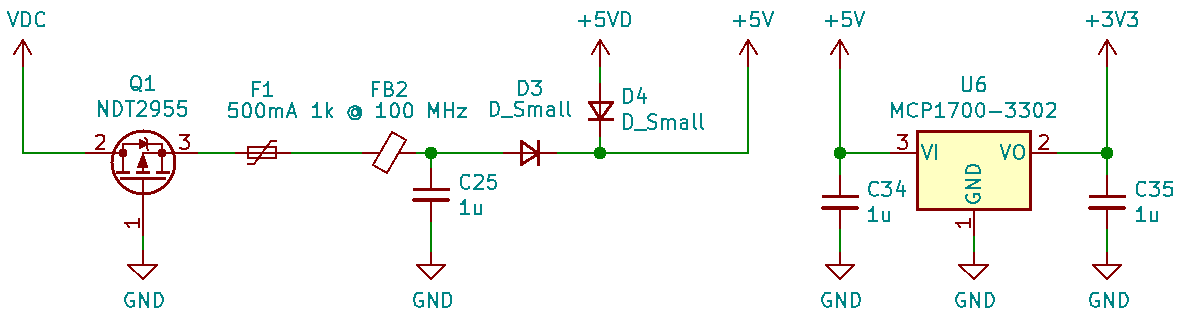
\includegraphics[width=0.9\textwidth]{obrazky/schem_power}
    \caption{The 5~V power rail for powering the MCU and peripherals.}
    \label{fig:power}
\end{figure}

\subsection{CAN Bus Circuitry}
\label{subsec:can_circuitry}
In order to transmit \acs{can} frames over the \acs{can} differential pair, a transceiver that converts digital signal from the \acs{mcu} to the differential signal needs to be utilized.
We utilized the MCP2562 transceiver because we needed it to support 3.3 V logic levels for the \acs{mcu} and 5 V levels for the differential pair and we also had previous experience with the transceiver.
In the future revisions, this transceiver will most likely be replaced by the newer MCP2562-FD transceiver as the currently used one is "Not Recommended for New Designs"\cite{microchip_mcp2562_nodate}.

The schematics of the transceiver circuits can be seen in the Figure~\ref{fig:schem_can}.
On the left, we can see a resistor network that can be utilized to support other transceivers as they are commonly pin-to-pin compatible except for the \textbf{Vio} and \textbf{STBY} pins that usually have different function.
On the right, we can see the bus termination resistor with a jumper and two connectors to connect the SM4 controller with other circuits.
The capacitors on the bottom are used for power rail filtering.

\begin{figure}[H]
    \centering
    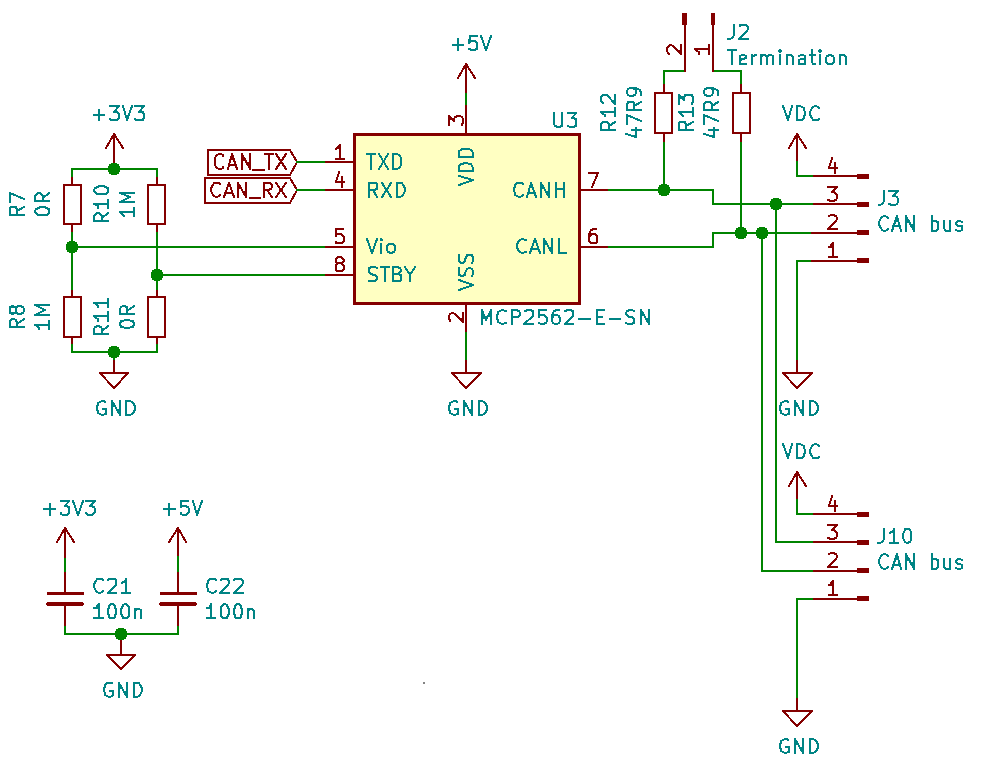
\includegraphics[width=0.9\textwidth]{obrazky/schem_can}
    \caption{The schematic of the CAN bus transceiver circuitry.}
    \label{fig:schem_can}
\end{figure}

\subsection{USB Circuitry}
\label{subsec:usb_circuitry}
For configuration and flashing purposes a USB connection was added.
The schematic for it can be found in the Figure~\ref{fig:schem_usb} and was inspired by the example project video\cite{salmony_kicad_2020}.
As can be seen in the schematic, there is not many external components required for the \acs{usb} to work, this is caused by the fact, that the correct passive components are contained directly in the \acs{mcu}.
According to the AN4879\cite{stmicro_an4879_2018}, the \acs{usb} peripheral already includes the \textbf{D+} pull-up resistor, so it is not required to be realized by an external component.
On the left, we can see an \acs{esd} (\acl{esd}) protection circuit, protecting the \acs{mcu} from electrostatic discharge caused by human contact on the connector.
It protects both the data lines and the VBUS.

On the right, we can see a USB-C\texttrademark receptacle.
In order to support USB-C\texttrademark reversibility, both data lines of the differential pairs are connected together.
A pull-down resistor with the value of 5.1~k\textohm was connected to both of the \textbf{CC} lines of the USB-C\texttrademark connector.
These resistors are used for device discovery, configuration and connection management over a USB-C\texttrademark cable and also for communication in case the device has the power USB Power Delivery\cite{stmicro_ta0357_2018}, which our device doesn't support.
As an additional protection measure a \acs{ptc} fuse is added to the VBUS power rail.

\begin{figure}[H]
    \centering
    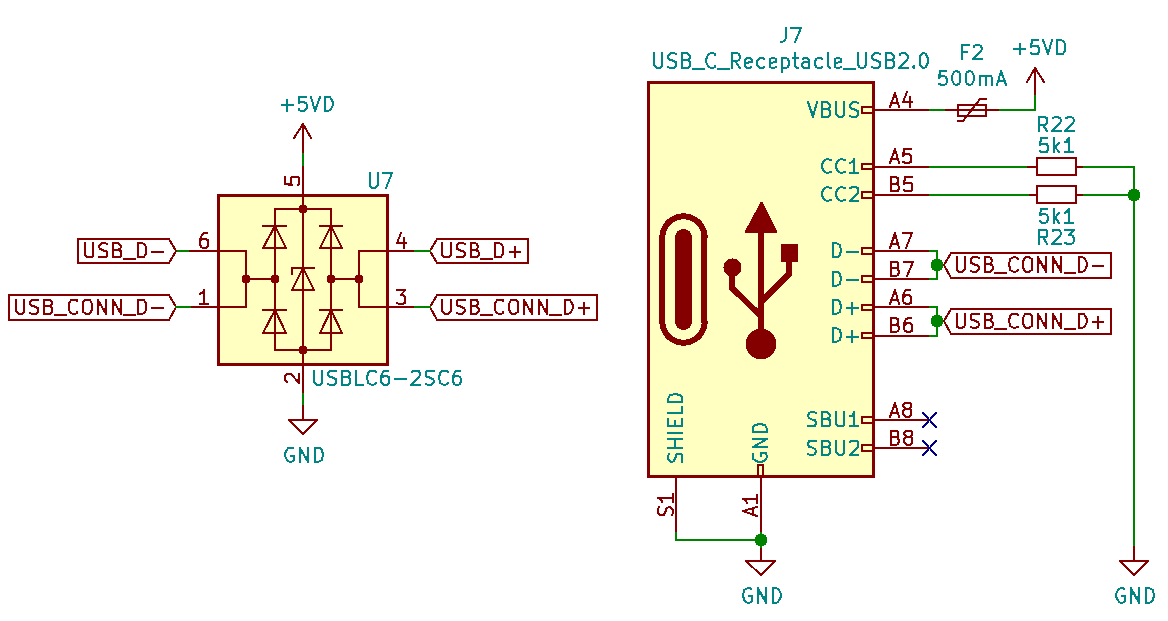
\includegraphics[width=0.9\textwidth]{obrazky/schem_usb}
    \caption{The schematic of the USB circuit.}
    \label{fig:schem_usb}
\end{figure}

\subsection{Stepper Driver Circuitry}
\label{subsec:stepper_circuitry}
There are two hardware revisions with two types of the stepper motor driver \acs{ic}s.
Both of the circuits were adapted from the \acs{ic} datasheet\cite{trinamic_tmc2100-datasheet_2018, trinamic_tmc2226_2020}.
The datasheet recommends motor voltage filtering using quite large electrolytic capacitors (100~\textmu F), in order to save vertical space, these capacitors were replaced using 10~\textmu F capacitors with maximal voltage of 50~V.

\subsubsection{Revision 1}
The schematic for the circuit of the first revision can be seen in the Figure~\ref{fig:schem_driver1}.
This revision utilized the TMC2100-TA driver \acs{ic}.
This driver is configured using \acs{gpio} and it is configured in the following way:
\begin{itemize}
    \item use internal sense resistor with \textbf{AIN} as current reference for internal sense resistors or use external sense resistors with \textbf{AIN} for scaling,
    \item use either SpreadCycle\texttrademark or StealthChop\texttrademark with interpolation and 16 microsteps,
    \item shortest slow decay phase,
    \item recommended chopper hysteresis - low hysteresis with 4\% of full scale current,
    \item shortest chopper blank time,
\end{itemize}
These values were chosen by following the recommended values from the datasheet.
In the schematic, which was adapted from the recommended schematic in the datasheet\cite{trinamic_tmc2100-datasheet_2018}, we can see motor power rail filtering capacitor composed from five 10~\textmu F capacitors, then there are some more filtering capacitors and capacitors for the integrated charge pump.
In the center of the schematic, there is the driver \acs{ic} itself.
The driver \acs{ic} is controlled using the \textbf{REF, EN, STEP, DIR} and \textbf{MODE} signals, to indicate for an error, the \textbf{ERR} signal is consumed by the \acs{mcu}.
The current sensing resistor values are set to 0.22~\textohm, allowing for driving motors with 0.96~A RMS phase current.

\begin{figure}[H]
    \centering
    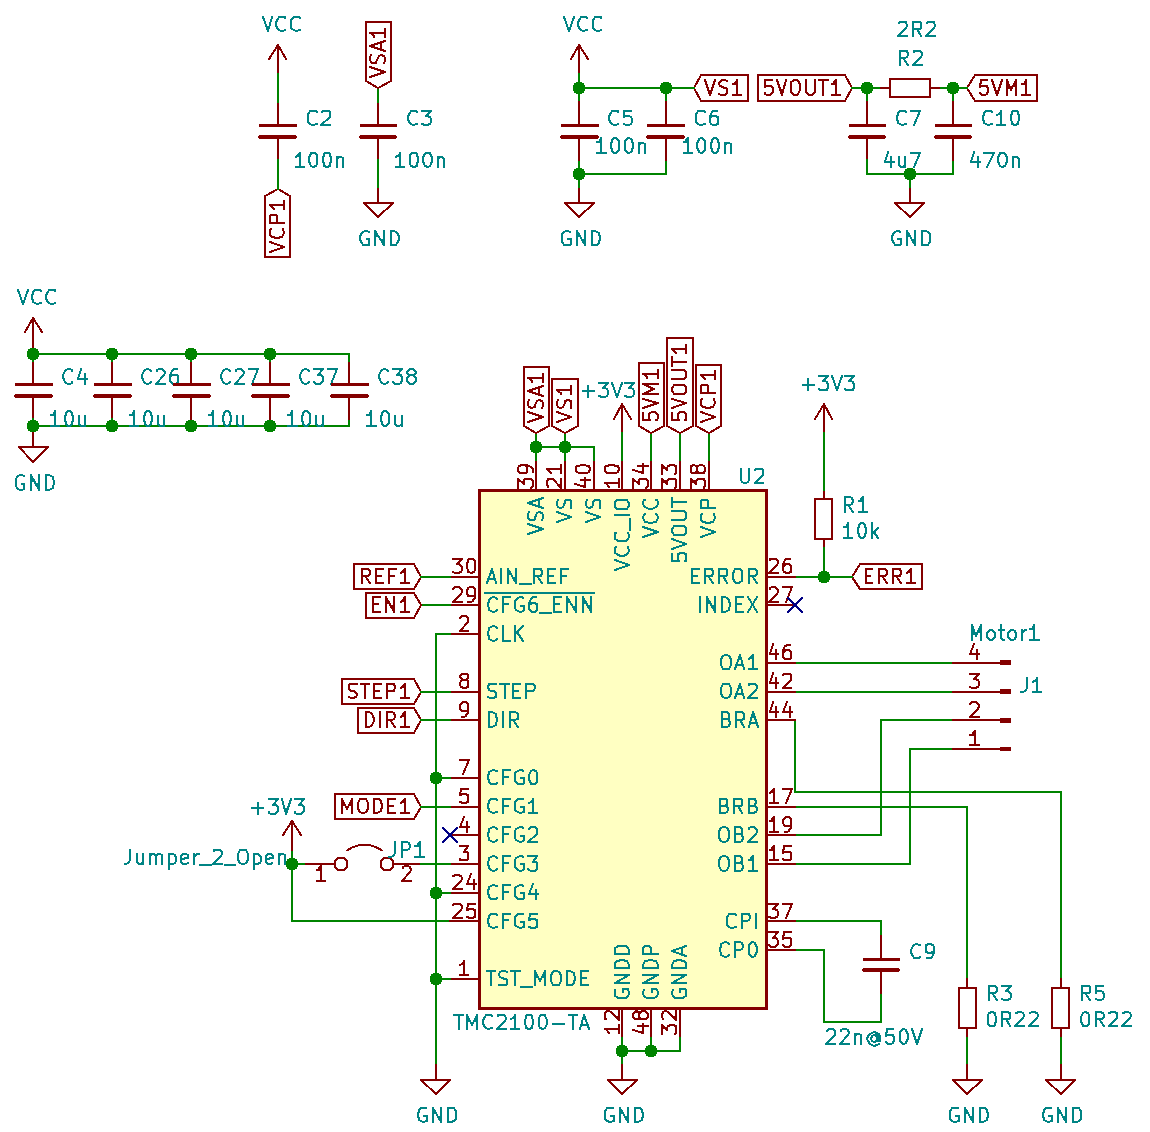
\includegraphics[width=0.95\textwidth]{obrazky/schem_driver_rev1}
    \caption{The schematic of the stepper motor driver IC in the first revision.}
    \label{fig:schem_driver1}
\end{figure}

\subsubsection{Revision 2}
In the Figure~\ref{fig:schem_driver2}, we can see the schematic of the second hardware revision with the TMC2226-SA stepper motor driver \acs{ic}.
On the top, we can see the motor power rail filtering capacitors and also some auxiliary capacitors required by the datasheet.
In the center there is the driver \acs{ic} itself, there are again some filtering capacitors and connections to the motor and to the \acs{mcu}.
To support multiple drivers on the same UART configuration interface, the driver's address need to be set using the \textbf{MS1\_AD0} and \textbf{MS2\_AD1} pins.
There are also some other configuration pins, but these have not been connected as their function can be replaced by the configuration interface.
For controlling the driver \acs{ic}, the \textbf{STEP} and \textbf{DIR} pins are utilized.
Finally, in the bottom right corner there are the current sensing resistors for the motor phases current.
Their value was chosen by the datasheet so support the maximal RMS phase current of 1.92 A - 0.1~\textohm.
It is important to select resistors with the proper power rating, in this case $P = R * I^2 = 0.1\Omega * (1.92 A)^2 = 0.4 W$, therefore we need resistors rated for at 0.5 W of power dissipation.

\begin{figure}[H]
    \centering
    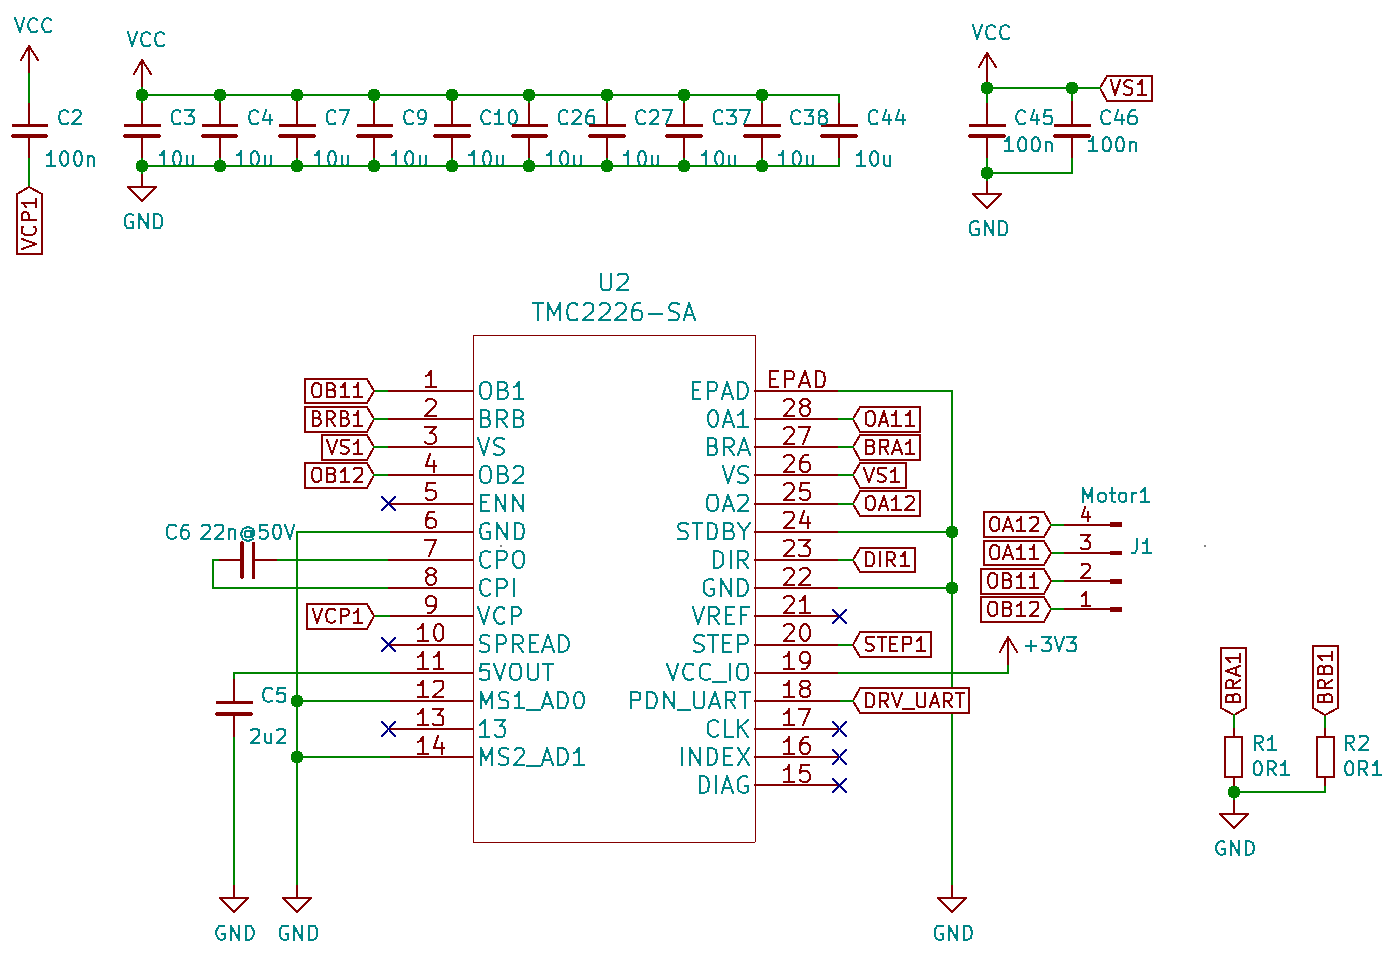
\includegraphics[width=\textwidth]{obrazky/schem_driver_rev2}
    \caption{The schematic of the stepper motor driver IC in the second revision.}
    \label{fig:schem_driver2}
\end{figure}

\subsection{Auxiliary Circuitry and Connectors}
\label{subsec:aux_connectors}
In order to improve the user experience, debugging and to make the controller future-proof a bit, we added some auxiliary circuits (shown in the Figure~\ref{fig:schem_aux}) and future-proofing connectors (shown in the Figure~\ref{fig:schem_enc_gpio}).

In the Figure~\ref{fig:schem_aux}, we can see that there are four \acs{led}s for debugging and indicating driver's state, two of them indicate power on the 3.3~V rail and on the motor power rail (VCC).
The other two \acs{led}s are connected to the \acs{mcu} and can be utilized to show status and error states of the SM4 driver.
Further, there is the voltage divider used for sensing the motor power rail voltage.
Apart from the two resistors, there is also a small filtering capacitor.
The resistor values were calculated for the first revision which aimed to support up to 43~V, given this voltage, the output voltage on the divider would be $U_{out} = U_{in} * \frac{R19}{R18+R19} = 43 V * \frac{4.7 k\Omega}{104.7 k\Omega} = 1.93 V$, which is small enough for the internal \acs{adc} of the \acs{mcu}.

In order to improve the user experience we also added I\textsuperscript{2}C pull-up resistors, that can be connected to the bus using solderable \acs{no} (\acl{no}) jumpers.
The values for these pull-up resistors was chosen 2.2 k\textohm, this is because we want to connect the driver using wires with unknown parasitic capacitance which can be compensated by lower resistance of the resistors.
Another reason is that the student boards have Zener diodes limiting the voltage on the I\textsuperscript{2}C bus lines and these diodes require quite high current to function properly.

\begin{figure}[H]
    \centering
    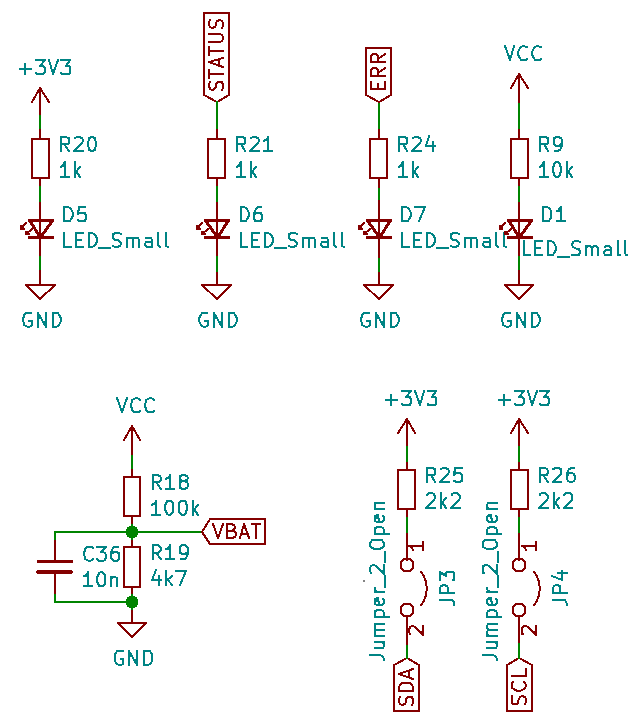
\includegraphics[width=0.5\textwidth]{obrazky/schem_aux}
    \caption{Auxiliary circuits schematic - LEDs, I\textsuperscript{2}C, motor voltage measurement.}
    \label{fig:schem_aux}
\end{figure}

We wanted to future-proof the SM4 driver and therefore we added three connectors which will enable expanding the controller in the future.
The connectors' schematic is depicted in the Figure~\ref{fig:schem_enc_gpio}.
The first connector on the left is a connector designed to add two incremental encoders to the stepper driver.
It supports quadrature encoders with index pulse.
The second connector in the middle is the \acs{gpio} connector, which can be used to expand the driver's capabilities using five logic signals.
Finally, on the right, there is a connector with two \acs{spi} buses broken out, which should allow for connecting SSI absolute encoders by bit-banging the SSI bus.

\begin{figure}[H]
    \centering
    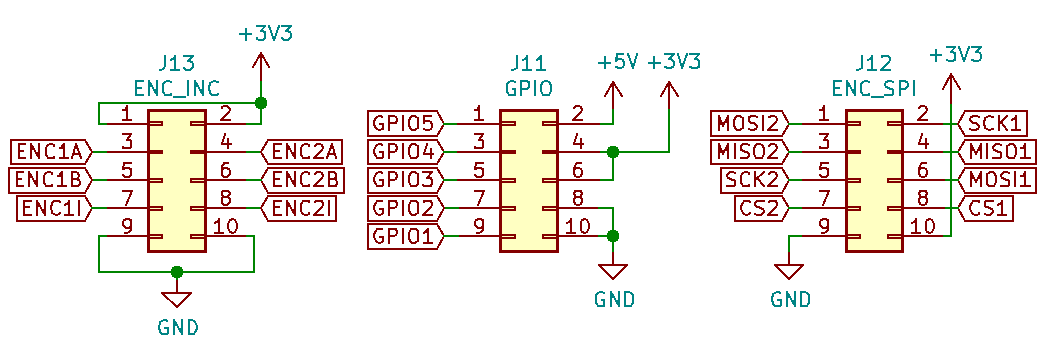
\includegraphics[width=0.9\textwidth]{obrazky/schem_enc_gpio}
    \caption{Schematic of connectors that allow for connecting incremental and absolute encoders and extending the driver with logic signals.}
    \label{fig:schem_enc_gpio}
\end{figure}

\subsection{PCB Design}
\label{subsec:pcb_design}
When the schematic design was done, we went on to route the \acs{pcb}.
As for the layer stackup, we utilized the four-layer one, with internal layers used for \acs{gnd} and 3.3~V routing and the outside layers for signals.
The stackup was previously described in the Section~\ref{subsec:hardware_design_choices}.
With trace widths and via sizes, we aimed for compatibility with the technologies provided by the JLCPCB manufacturing house, but with some margin to be safe there are not problems with manufacturing, which meant 0.2~mm minimal trace width and 0.8~mm wide vias, with 0.4~mm via drill size.
Given limitations with the assembly service, all of the components are placed on the top side of the \acs{pcb}.
The \acs{pcb} was designed to fit the area on the Raspberry Pi behind the ethernet and \acs{usb} ports and is therefore 65x56~mm.
When designing we also aimed to have the power and communication connectors along a single side of the \acs{pcb} and connectors for the motors on another one.
The final \acs{pcb} design for both of the revisions can be seen in the Figures~\ref{fig:pcb1} and~\ref{fig:pcb2}.

\begin{figure}[H]
    \begin{minipage}[t]{0.45\textwidth}
        \centering
        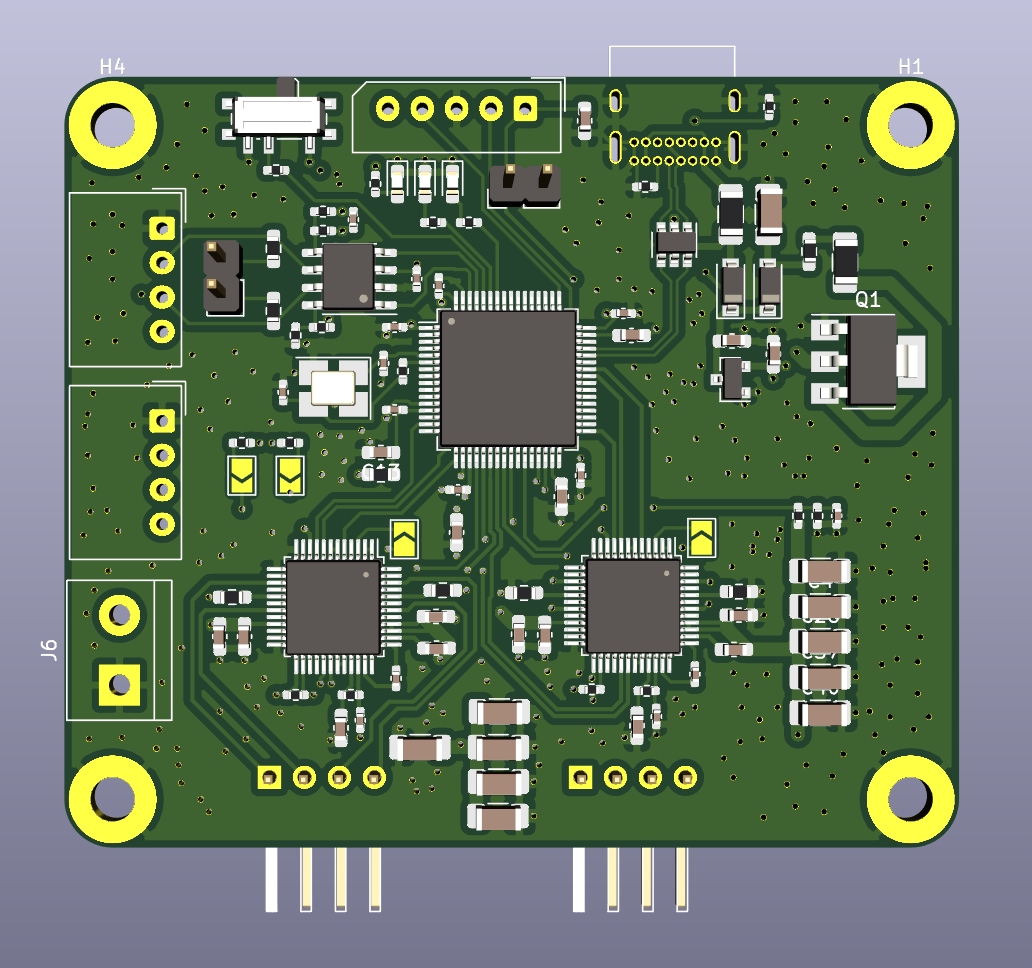
\includegraphics[width=0.9\textwidth]{obrazky/pcb_rev1}
        \caption{Rendered first revision PCB.}
        \label{fig:pcb1}
    \end{minipage}\hfill
    \begin{minipage}[t]{0.45\textwidth}
        \centering
        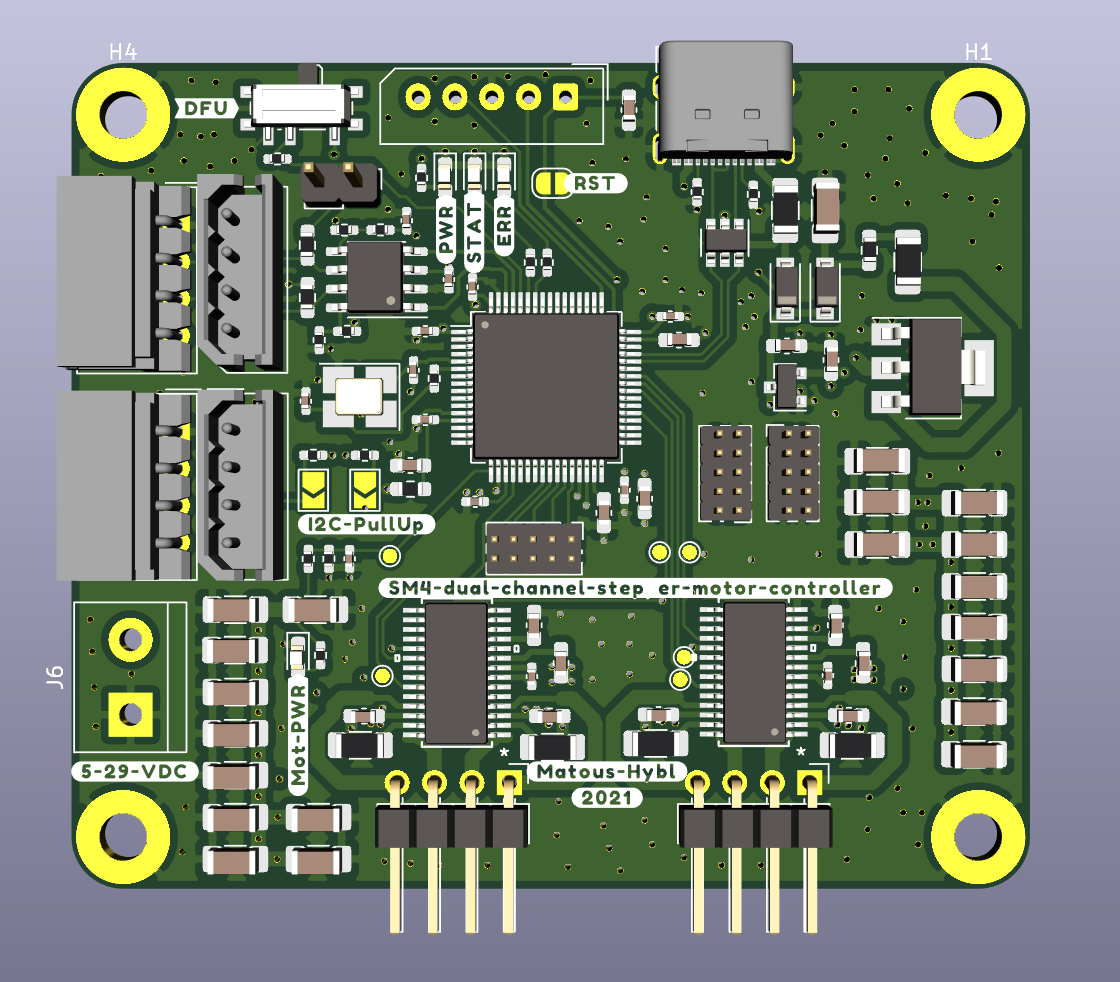
\includegraphics[width=0.9\textwidth]{obrazky/pcb_rev2}
        \caption{Rendered second revision PCB.}
        \label{fig:pcb2}
    \end{minipage}
\end{figure}
